% !TEX root = CSL 2021.tex

To illustrate our construction, we start from a relatively concrete example: we consider a simply-typed lambda calculus with a base type and primitives for real numbers, and we follow the plan outlined in the introduction, which yields for each simple type a notion of interval, of approximate function, diameter and distance between programs. Most definitions are rather intuitive: the interesting, not immediately obvious point is that our construction does yield a \emph{partial metric} on each type.

\emph{Simple types} are defined as follows: $\mathsf{Real}$ is a simple type; if $A$ and $B$ are simple types, then $A \to B$ and $A \times B$ are simple types.

For all $n>0$, we fix a set $\mathcal{F}_n$ of functions from $\mathbb{R}^n$ to $\mathbb{R}$. We consider the usual Curry-style simply-typed $\lambda$-calculus $\STLC$ over the types defined above (the left and right projection are denoted by $\pi_L:A\times B \to A$ and  $\pi_R:A\times B \to B$ respectively, and the constructor for pairs by $\left\langle-,-\right\rangle$), enriched with the following constants: for all $r \in \mathbb{R}$, a constant $r:\mathsf{Real}$; for all $n>0$ and all $f\in\mathcal{F}_n$, a constant $f:\mathsf{R}\to\ldots\to\mathsf{R}\to\mathsf{R}$. The terms of this calculus are simply called \emph{terms}. We write $t[x_1 := u_1, \ldots, x_n := u_n]$ to denote the \emph{simultaneous} substitution of $u_1, \ldots, u_n$ for $x_1, \ldots, x_n$ in $t$. For all types $A$, we denote by $\Lambda_A$ the set of closed terms of type $A$. The relation of $\beta$-reduction is enriched with the following rule, extended to all contexts: for all $n>0$, $f\in\mathcal{F}_n$, and $r_1,\ldots,r_n\in\mathbb{R}$, $f r_1 \ldots r_n \to_\beta s$, where $s = f(r_1, \ldots, r_n)$. By standard arguments, this calculus has the properties of subject reduction, confluence and strong normalisation.


Given two closed terms $t,u$ of type $A$,  we say that $t$ and $u$ are \emph{observationally equivalent} and write $t \oeq_A u$, if for all terms $C$ such that $x:A \vdash C : \mathsf{Real}$ is derivable, $C[x:=t]$ is $\beta$-equivalent to $C[x:=u]$ (which amounts to saying that they both $\beta$-reduce to the same real number).  It is clear that observational equivalence is a congruence and that two $\beta$-equivalent terms are always observationally equivalent. The notion of distance we define in the next paragraph will be a generalisation of this notion of equivalence.



\subsection{Approximate values and approximate programs}

The first step of our construction for $\STLC$ is to associate to each simple type $A$ a set $\intervals{A}$ whose elements are certain sets of programs of type $A$ that we call \emph{approximate values of type $A$}. 
A closed term $t\in \Lambda_{A}$ represents a program with return type $A$ and no parameters, so an approximate value can be thought as a specification of a program with return type $A$ and no parameters \emph{up to} a certain degree of error or approximation.

For each simple type $A$, the set of approximate values $\intervals{A}\subseteq \mathcal P(\Lambda_A)$ is defined inductively as follows:
\begin{itemize}
\item $\intervals{\mathsf{Real}} = \{ \{ t \in \Lambda_\mathsf{Real} \mid \exists r \in I, t \to_\beta^* r \} \mid I \subseteq \mathbb{R} \text{ is a compact interval or $\emptyset$ or } \mathbb{R} \}$,
\item $\intervals{A \times B} = \{ \{ t \in \Lambda_{A \times B} \mid \pi_L t \in a \text{ and } \pi_R t \in b \} \mid a  \in \intervals{A}, b \in \intervals{B} \}$,
\item $\intervals{A \to B} = \{ \{ t \in \Lambda_{A \to B} \mid \forall u \in \Lambda_{A},~ tu \in I(u) \} \mid I : \Lambda_A \to \intervals{B} \}$.
\end{itemize}

The approximate values of type $\mathsf{Real}$ essentially coincide with the compact intervals of $\mathbb R$, plus the empty set and $\mathbb{R}$ itself. An approximate value in $\intervals{A\times B}$ is uniquely determined by a pair of approximate values $(a,b)$, with $a\in \intervals{A}$ and $bs\in \intervals{B}$, while an approximate value in $\intervals{A\to B}$ is uniquely determined by a function 
$I$ from closed terms $u\in \Lambda_{ A}$ to approximate values $I(u)\in \intervals{B}$.

For example, any two terms $t,u\in \Lambda_{\mathsf{Real}}$ with normal forms $q,r\in \mathbb{R}$ induce an approximate value of type $\mathsf{Real}$ $[t,u]_{\mathsf{Real}}= \{v\in \Lambda_{\mathsf{Real}}\mid  v\to_{\beta}^{*} s \land q\leq s\leq r\}$. Similarly, any two terms $t,u\in \Lambda_{\mathsf{Real}\to \mathsf{Real}}$ induce an approximate value
$[t,u]_{\mathsf{Real}\to \mathsf{Real}}= \{v\in \Lambda_{\mathsf{Real}\to\mathsf{Real}}\mid  
\forall r \in \Lambda_{\mathsf{Real}} \ vr\in [ tr, ur]_{\mathsf{Real}} 
\}$. With $t= \lambda x.\sin(x)+1$ and $u=\lambda x.\cos(x)-1$, 
$[t,u]_{\mathsf{Real}\to \mathsf{Real}}$ contains all closed terms corresponding to maps oscillating between $\sin (x)+1$ and $\cos(x)+1$ (\textit{e.g.} $\lambda x. \sin(x+1)$, as illustrated in Fig. \ref{fig:interval1}).

\begin{figure}
\begin{subfigure}{0.42\textwidth}
\parbox[h][3cm][c]{\textwidth}{
\adjustbox{center}{$
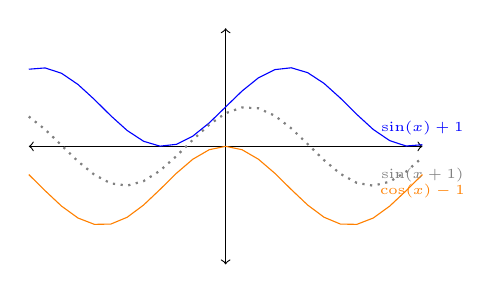
\begin{tikzpicture}[domain=-5:5, scale=0.5]
%\draw[very thin,color=gray] (-0.1,-1.1) grid (3.9,3.9);
\draw[<->]   (-5,0) -- (5,0);
\draw[<->] (0,-3) -- (0,3); % node[above] {$f(x)$};

   % \node at (0,0)[circle,fill,inner sep=1pt]{};
%
\draw[color=blue] plot (\x,{sin(\x r)+1}) node[above] {\tiny$\sin(x)+1$};
\draw[color=orange] plot (\x,{cos(\x r)-1}) node[below] {\tiny$\cos(x)-1$};

\draw[color=gray, dotted, thick] plot (\x,{sin(deg(\x+1) ))}) node[below] {\tiny$\sin(x+1)$};


\end{tikzpicture}$}
}
\caption{\small $\lambda x.\sin(x+1)$ is in $[\lambda x.\sin(x)+1, \lambda x.\cos(x)+1]_{\mathsf{Real}\to\mathsf{Real}}$.}
\label{fig:interval1}
\end{subfigure} \ \ \ 
\begin{subfigure}{0.52\textwidth}
\parbox[h][3cm][c]{\textwidth}{
\adjustbox{center}{$
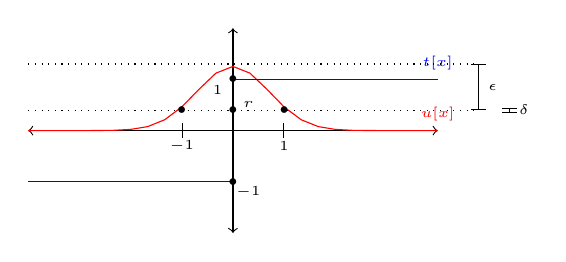
\begin{tikzpicture}[domain=-4:4, scale=0.65]

%\draw[very thin,color=gray] (-0.1,-1.1) grid (3.9,3.9);
\draw[<->]   (-4,0) -- (4,0);
\draw[<->] (0,-2) -- (0,2); % node[above] {$f(x)$};

\draw[dashed, |-|] (-1,0) -- (1,0);
\node(a) at (-1,-0.3) {\tiny$-1$};
\node(a) at (1,-0.3) {\tiny$1$};

\node(a) at (0.3,-1.2) {\tiny$-1$};
\node(a) at (-0.3,0.8) {\tiny$1$};
   % \node at (0,0)[circle,fill,inner sep=1pt]{};

\draw[|-|] (4.8,0.4) -- node[right] {\tiny$\epsilon$} (4.8,1.3);

\draw[|-|] (5.4,0.35) -- node[right] {\tiny$\delta$} (5.4,0.45);


\draw[color=red, domain=-4:4] plot (\x, {(1/2*sqrt(2*pi))*exp(-((\x)^2)) } ) node[above] {\tiny$u[x]$};
%\draw[color=violet, domain=-1.2:1.2] plot (\x, { (\x)^3 } );

\draw[color=blue, domain=-4:0] plot (\x,-1);
\draw[color=blue, domain=0:4] plot (\x,1) node[above] {\tiny$t[x]$};

\draw[dotted] (-4,0.4) -- (4.8,0.4);
\draw[dotted] (-4,1.3) -- (4.8,1.3);

\node(z) at (-1,0.4) {\tiny$\bullet$};
\node(zz) at (1,0.4) {\tiny$\bullet$};

\node(z) at (0,-1) {\tiny$\bullet$};
\node(zz) at (0,1) {\tiny$\bullet$};

\node(r) at (0,0.4) {\tiny$\bullet$};
\node(rr) at (0.3,0.5) {\tiny$r$};



\end{tikzpicture}$}
}
\caption{\small $\epsilon=(\partial(u)\circ \partial(t))([-1,1])$ is bigger than $\delta=\partial(u\circ t)([-1,1])=[r,r]$.}
\label{fig:interval2}
\end{subfigure}
\end{figure}

For all $A$, as a subset of $\mathcal{P}(\Lambda_A)$, $\intervals{A}$ is closed under arbitrary intersections and is therefore a complete lattice whose meet is given by intersection. In particular, for all $t\in\Lambda_A$, there is a least element of $\intervals{A}$ that contains $t$, which will be denoted by $\tointerval{t}$. 
One can check that $\tointerval{t} = \tointerval{u}$ if and only if $t\oeq_{A} u$.

Monotone functions from approximate values to approximate values represent \emph{approximate programs}. They behave like a model of simply-typed $\lambda$-calculus in a weak sense, namely: \begin{itemize}
\item for all monotone functions $(x_1, \ldots, x_n) \mapsto c[x_1, \ldots, x_n] : \intervals{A_1} \times \ldots \times \intervals {A_n} \to \intervals {B \to C}$ and $(x_1, \ldots, x_n) \mapsto b[x_1, \ldots, x_n] : \intervals{A_1} \times \ldots \times \intervals {A_n} \to \intervals {B}$, we can define a monotone function $(x_1, \ldots, x_n) \mapsto c[x_1, \ldots, x_n]~ b[x_1, \ldots, x_n] = \sup\{\tointerval{vu} \mid v \in c[x_1, \ldots, x_n], u \in b[x_1, \ldots, x_n]\} : \intervals{A_1} \times \ldots \times \intervals {A_n} \to \intervals {C}$,
\item for all monotone functions $(x_1, \ldots, x_n) \mapsto c[x_1, \ldots, x_n] : \intervals{A_1} \times \ldots \times \intervals {A_n} \to \intervals {C}$ and all $i \leq n$, we can define a monotone function $(x_j)_{j \neq i} \mapsto \lambda x_i.~ c[x_1, \ldots, x_n] = \{ v \in \Lambda_{A_i \to C} \mid \forall t_i \in \Lambda_{A_i},~ v t_i \in c[x_1, \ldots, \tointerval{t_i}, \ldots, x_n] \} : \prod_{j \neq i} \intervals{A_j} \to \intervals{A_i \to C}$,
\end{itemize}
and these two constructions are weakly compatible with $\beta$-reduction and $\eta$-expansion:

\begin{proposition} \label{prop:intervals-weak-model-lambda} For all monotone functions $(x_1, \ldots, x_n, y) \mapsto c[x_1, \ldots, x_n, y] : \intervals{A_1} \times \ldots \times \intervals {A_n} \times  \intervals {B} \to \intervals {C}$ and $(x_1, \ldots, x_n) \mapsto b[x_1, \ldots, x_n] : \intervals{A_1} \times \ldots \times \intervals {A_n} \to \intervals {B}$, $$\begin{array}{ll} & (x_1, \ldots, x_n) \mapsto (\lambda y.~  c[x_1, \ldots, x_n, y])~ b[x_1, \ldots, x_n] \\ \leq & (x_1, \ldots, x_n) \mapsto c[x_1, \ldots, x_n, b[x_1, \ldots, x_n]]\text{,}\end{array}$$
and for all monotone functions $(x_1, \ldots, x_n) \mapsto d[x_1, \ldots, x_n] : \intervals{A_1} \times \ldots \times \intervals {A_n} \to  \intervals {B \to C}$,
$$\begin{array}{ll} & (x_1, \ldots, x_n) \mapsto \lambda y.~  d[x_1, \ldots, x_n]~ y \\ \geq & (x_1, \ldots, x_n) \mapsto d[x_1, \ldots, x_n]\text{,}\end{array}$$
where functions are ordered by pointwise inclusion.  In other words, on approximate programs, $\beta$-reduction and $\eta$-expansion \emph{discard} information, and conversely $\beta$-expansion and $\eta$-reduction \emph{recover} some information.
\end{proposition}

\begin{proof} Without loss of generality, we can assume $n=0$.

Let $v \in \lambda y.~ c[y]$ and $u \in b$. By definition, $tu \in c[\tointerval{u}]$, so $\tointerval{tu} \subseteq c[\tointerval{u}] \subseteq c[b]$. Therefore, $(\lambda y.~ c[y])~ b \subseteq b$.

Let $v \in d$. For all $u \in \Lambda_B$, by definition, $vu \in d\tointerval{u}$. Therefore, $v \in \lambda y.~ d~ y$.
\end{proof}

In addition, we can define a weak embedding from terms into approximate programs, by mapping each term to its tightest approximation: for all terms $t$ such that $x_{1}:A_{1},\dots,x_{n}:A_{n}\vdash t:B$, we define a monotone function $\partial(t):\intervals{A_{1}}\times \dots \times \intervals{A_{n}} \to \intervals{B}$ by $\partial(t)(a_1, \ldots, a_n) = \sup \{ \tointerval{t u_1 \ldots u_n} \mid u_1 \in \intervals{A_1}, \ldots, u_n \in \intervals{A_n} \}$. The map $\partial$ is constant on classes of observational equivalence, and one can check that it is is weakly compatible with the constructions of the $\lambda$-calculus, namely:
\begin{itemize}
\item $\partial (x_{i})(a_{1},\dots, a_{n})=a_{i}$,
\item $\partial (tu)(a_{1},\dots, a_{n}) \subseteq \partial (t)(a_{1},\dots, a_{n}) ~ \partial (u)(a_{1},\dots, a_{n})$,
\item $\partial (\lambda x. t)(a_{1},\dots, a_{n}) \subseteq \lambda x.~ \partial (t)(x, a_{1},\dots, a_{n})$.
\end{itemize}

This map $\partial(t)$ can be taken as a measure of the \emph{sensitivity} of $t$, as it maps an interval $a$, that is a quantifiably uncertain input, to a quantifiably uncertain output $\partial(t)(a)$. 
For instance, if we take the term $t[x]= \sin(x)+1$ above, then $\partial(t): \intervals{\mathsf{Real}}\to \intervals{\mathsf{Real}}$ sends the interval $[-\pi,\pi]_{\mathsf{Real}}$ into $[0,2]_{\mathsf{Real}}$.

\begin{remark}
When composing two maps $\partial(t)$ and $\partial(u)$, we might obtain a worse approximation than by computing $\partial(t[u/x])$.
For instance, let $t[x]$ and 
$u[x]$ be, respectively, the discontinuous and Gaussian functions illustrated in Fig. \ref{fig:interval2}.  
If $a$ is the interval $[-1,+1]$, then $\partial(t)(a)=[-1,1]$, and since $u[x:=-1]=u[x:=1]\simeq_{\beta} r$, for some $0<r<1$, we deduce $\partial(u)(\partial(t)(a))=[-1,1] \supset [r,r  ]= \partial (u[t/x])(a)$.

\end{remark}










\subsection{A partial metric on each type}

We will now show how to associate to each type $A$ of $\STLC$ a partial metric space $(\Lambda_{A}/\oeq_{A}, \distances{A}, d_{A})$. The definition of this space will exploit in an essential way the sets of intervals $\intervals{A}$.


For all simple types $A$, we define a commutative integral quantale $(\distances{A}, \quantaleleq_A, \quantaleop_A)$ of \emph{distances of type $A$}:
\begin{itemize}
\item $(\distances{\mathsf{Real}}, \quantaleleq_\mathsf{Real}, \quantaleop_\mathsf{Real}) = ([0,\infty], \geq, +)$ (note the reversed ordering),
\item $\distances{A \times B} = \distances{A} \times \distances{B}$ with the product ordering and the product monoid operation,
\item $\distances{A \to B} = \{ \text{monotonically decreasing functions from } \intervals{A} \text{ to } \distances{B} \}$, with the pointwise ordering and the pointwise monoid operation.
\end{itemize}
It is straightforward to check that this does indeed define a commutative integral quantale.

For all simple types $A$, we define a \emph{distance function} $d_A : \Lambda_A \times \Lambda_A \to \distances{A}$:
\begin{itemize}
\item $d_\mathsf{Real}(t,u) = \left\vert r-s \right\vert$, where $r,s$ are the unique elements of $\mathbb{R}$ such that $t \to_\beta^* r$ and $u \to_\beta^* s$,
\item $d_{A \times B}(t,u) = (d_A(\pi_L t, \pi_L u), d_B(\pi_R t, \pi_R u))$,
\item $d_{A \to B}(t,u) = a \mapsto \inf \left\{ d_B(tv, uw) \mid v,w \in a \right\}$.
\end{itemize}

This distance is clearly compatible with observational equivalence (\textit{i.e.} if $a \oeq_A a'$ and $b \oeq_A b'$, then $d_A(a,b) = d_A(a',b')$). Our objective is now to prove that $\left(\Lambda_A/\oeq_A, \distances{A}, d_A\right)$ is a partial metric space.


To this end, we define for all simple types $A$ a monotonically decreasing \emph{diameter function} $\diam_A : \intervals{A} \to \distances{A}$ by $\diam_A(a) = \inf \{ d_A(t,u) \mid t,u \in a \}$, and we exploit the fact that, as in the case of the reals (see [TODO: INTRODUCTION]), this diameter function $\diam_{A}$ is (almost) submodular on approximate values (or rather, using the quantale ordering convention, supermodular). First, one can check that for all $t,u \in \Lambda_A$, $\diam_A\left(\tointerval{t} \vee \tointerval{u}\right) = d_A(t,u)$, and that:
\begin{itemize}
\item $\diam_\mathsf{Real}(a) = \sup\{s-r \mid s,r \in \mathbb{R} \text{ such that } s,r \in a\}$,
\item $\diam_\mathsf{A \times B}(p) = \left(\diam_A\left(\sup\left\{\tointerval{\pi_L t} \mid t \in p\right\}\right), \diam_B\left(\sup\left\{\tointerval{\pi_R t} \mid t \in p\right\}\right)\right)$,
\item $\diam_\mathsf{A \to B}(b) = a \mapsto \diam_B\left(\sup\left\{\tointerval{vt} \mid t\in a, v \in b\right\}\right).$
\end{itemize}

With that, we can prove that the diameter function $\diam_{A}$ satisfies the following condition of ``quasi-supermodularity'':
\begin{proposition} For all simple types $A$ and all $a,b \in \intervals{A}$ such that $a \wedge b \neq \emptyset$, $\diam(a \wedge b) \quantaleop \diam(a \vee b) \quantalegeq \diam(a) \quantaleop \diam(b)$.
\end{proposition}
\begin{proof}
We proceed by induction on types.

Let $a,b \in \intervals{\mathsf{Real}}$ such that $a\wedge b \neq \emptyset$. Let $I = \{r \in \mathbb{R} \mid r \in a\}$ and $J = \{s \in \mathbb{R} \mid s \in b\}$: then $I$ (respectively, $J$, $I \cap J$, $I \cup J$) is either $\mathbb{R}$ or a non-empty compact interval of $\mathbb{R}$, and its length in the usual sense is equal to $\diam_\mathsf{Real}(a)$ (respectively, $\diam_\mathsf{Real}(b)$, $\diam_\mathsf{Real}(a \wedge b)$, $\diam_\mathsf{Real}(a \vee b)$). Note that $I \cup J$ is only an interval because $a\wedge b \neq \emptyset$ implies $I \cap J \neq \emptyset$. The length of an interval of $\mathbb{R}$ is equal to its Lebesgue measure, therefore $\operatorname{length}(I \cap J) + \operatorname{length}(I \cup J) = \operatorname{length}(I) + \operatorname{length}(J)$, so $\diam_\mathsf{Real}(a \wedge b) \quantaleop \diam_\mathsf{Real}(a \vee b) = \diam_\mathsf{Real}(a) \quantaleop \diam_\mathsf{Real}(b)$.

Let $a,b \in \intervals{A_L \times A_R}$ such that $a\wedge b \neq \emptyset$. For all $c \in \intervals{A_L \times A_R}$, let $c_L = \sup\{\tointerval{\pi_L t} \mid t \in c\}$ and $c_R = \sup\{\tointerval{\pi_R t} \mid t \in c\}$.
One can check that $(a \wedge b)_L = a_L \wedge b_L$, $(a \wedge b)_R = a_R \wedge b_R$, $(a \vee b)_L = a_L \vee b_L$ and $(a \vee b)_R = a_R \vee b_R$, so $\diam(a \wedge b) \quantaleop \diam(a \vee b) = (\diam(a_L \wedge b_L) \quantaleop \diam(a_L \vee b_L),  \diam(a_R \wedge b_R) \quantaleop \diam(a_R \vee b_R)) \quantalegeq (\diam(a_L) \quantaleop \diam(b_L), \diam(a_R) \quantaleop \diam(b_R)) = \diam(a) \quantaleop \diam(b)$.

Let $f,g \in \intervals{A \to B}$ and $a \in \intervals{A}$. For all $h \in \intervals{A \to B}$, let $ha = \sup\{\tointerval{vt} \mid v \in h, t \in a\}$. One can check that $(f \wedge g)a \subseteq (f a) \wedge (g a)$ and $(f \vee g)a = (f a) \vee (g a)$. As a result, $(\diam(f \wedge g)\quantaleop \diam(f \vee g))(a) \quantalegeq \diam((fa) \wedge (ga)) \quantaleop \diam((fa) \vee (ga)) \quantalegeq \diam(fa) \quantaleop \diam(ga) = (\diam(f)\quantaleop\diam(g))(a)$.
\end{proof}

\begin{corollary} \label{corollary:stlc-metric} For all simple types $A$, $\left(\Lambda_A/\oeq_A, \distances{A}, d_A\right)$ is a partial metric space, that is to say:
\begin{enumerate}
\item for all $t,u \in \Lambda_A$, $d_A(t,t) \quantalegeq d_A(t,u)$,
\item for all $t,u \in \Lambda_A$, if $d_A(t,t) = d_A(t,u) = d_A(u,u)$, then $t \oeq_A u$,
\item for all $t,u \in \Lambda_A$, $d_A(t,u) = d_A(u,t)$,
\item for all $t,u,v \in \Lambda_A$, $d_A(t,v) \quantaleop d_A(u,u) \quantalegeq d_A(t,u) \quantaleop d_A(u,v)$.
\end{enumerate}
\end{corollary}
\begin{proof}
As mentioned above, for all $t,u\in\Lambda_A$, $d_A(t,u) = \diam_A(\tointerval{t} \vee \tointerval{u})$, which immediately gives point 3. Since $\delta_A$ is monotonically decreasing and $\tointerval{t} \vee \tointerval{t} \leq \tointerval{t} \vee \tointerval{u}$, we also get point 1.

One can check (by induction on types) that the restriction of $\diam_A$ to the ideal generated by the $\tointerval{t}$ (for $t \in \Lambda_A$) is \emph{strictly} decreasing. Therefore, if  $d_A(t,t) = d_A(t,u) = d_A(u,u)$, \textit{i.e.} $\diam_A(\tointerval{t}) = \diam_A(\tointerval{t} \vee \tointerval{u}) = \diam_A(\tointerval{u})$,  then $\tointerval{t} = \tointerval{t} \vee \tointerval{u} = \tointerval{u}$, so $t \oeq_A u$.

The triangular inequality is an immediate consequence of the quasi-supermodularity of $\diam_A$: $d(t,v) \quantaleop d(u,u) = \diam(\tointerval{t} \vee \tointerval{v}) \quantaleop \diam(\tointerval{u}) \quantalegeq \diam((\tointerval{t} \vee \tointerval{u}) \vee (\tointerval{u} \vee \tointerval{v})) \quantaleop \diam((\tointerval{t} \vee \tointerval{u}) \wedge (\tointerval{u} \vee \tointerval{v})) \quantalegeq \diam(\tointerval{t} \vee  \tointerval{u}) \quantaleop \diam(\tointerval{u} \vee  \tointerval{v}) = d(t,u) \quantaleop d(u,v)$.
\end{proof}



















